\chapter{Architectural implementation}
\label{chap:archimpl}
 
In this chapter we will dig into the actual architectural implementation, seeing
all the problems related to it and how they were solved. We will show all the
various attemps made, and we will discussion about the technological issue and
changes we had to perform.

\section{First attempt}

In our first attempt we started building our infrastructure on top of Ubuntu
16.04 (for Openstack) and Ubuntu 18.04 (for Openbaton). Our main goal was to set
up Openstack as our VIM while setting Openbaton as our MANO. Then, Openbaton
would have Openstack registered as PoP, where TOSCA definition would be launched
on Openstack that, instead of deploying hypervisor based virtual machines, it
would have deployed container instances. The VNF lifecycles would have been
controller through an Element Management System (EMS), transmitting the various
VNF states via the message broker RabbitMQ. Is possible to see the interactions
between elements in a minimum schema available in
Figure~\ref{chap:archimpl:sec:fistattempt:img:schema1}.

\begin{figure}[t]
  \centering
  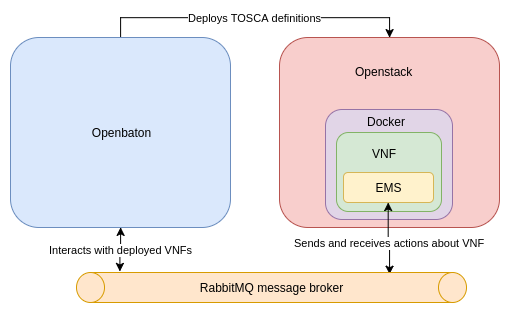
\includegraphics[scale=0.5]{Attempt1}
  \caption[Fist attempt components organization schema]{Fist attempt components
    organization schema. We can see how the main Openstack role is to deploy and
    manage the resources, while Openbaton has the role of maangement and
    orchestration. Finally, RabbitMQ sends and receives status update from the
    EMS for every VNF deployed.}
  \label{chap:archimpl:sec:fistattempt:img:schema1}
\end{figure}

\subsection{Adopting Openstack for container orchestration}

Our first step was to try to use Openstack to create a container orchestration. 
The reason behind this approach was simple: Openbaton, on paper, comes with an 
out-of-the-box support for Openstack. In fact, it natively supports Openstack 
PoPs, giving to us a great possibility to reuse the two frameworks and to ease 
the development phase of our software.
\subsubsection{Openstack for developers: Devstack}
Openstack is composed by modules, giving the possibility to the user who wants 
to install it to choose only the components it really needs. So the first thing 
we decided was to perform a selection of these modules between the 33 available 
in the installation page. The installation of this components span between 
multiple machines (nodes), therefore creating a whole cluster of resources. 
Since we considered too time-consuming to install Openstack in a distribuited 
manner, we considered to test first the developer version, called 
\emph{Devstack}. Devstack offers the possibility to install a subset of modules 
in the local machine, and to leverage a Openstack environment able to perform 
the same operations of the production-grade installation. Thus, we starting 
configurating the Devstack installation, installing first of all the Nova 
module, that is required to perform computer operations such as the launch of 
virtual machines, and lately we installed Tacker too.

\paragraph*{Taker}
\begin{figure}[h]
  \centering
  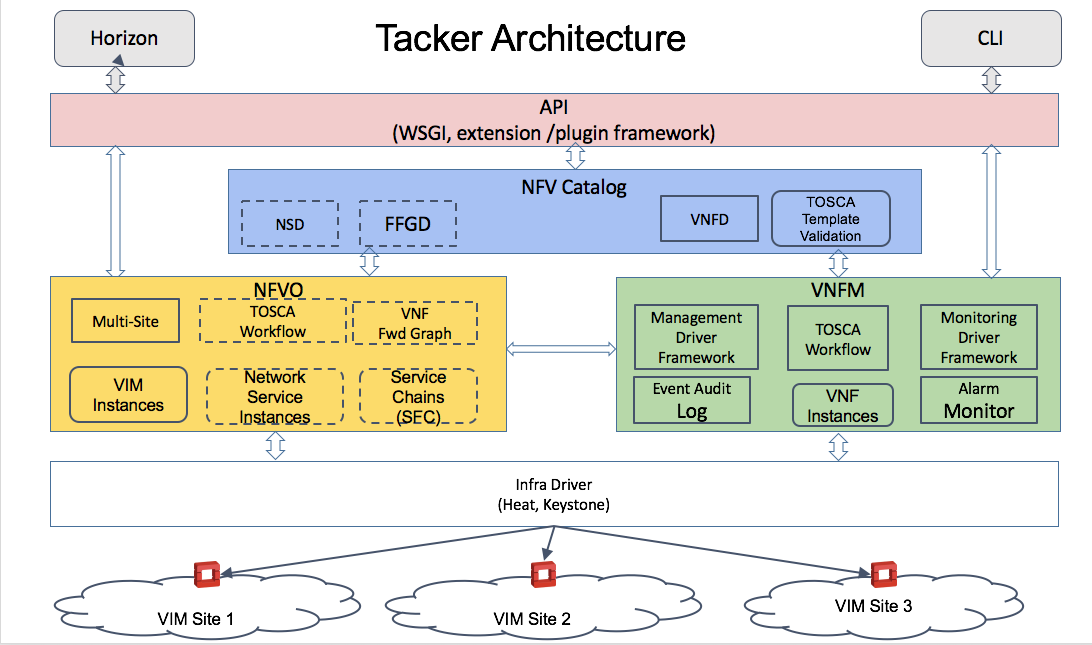
\includegraphics[scale=0.3]{tacker_architecture}
  \caption[Taker architecture schema]{Taker architecture
    schema~\cite{tackerOpenstackwiki}}
\end{figure}
Tacker is a VNFM and a NFVO. It is an official Openstack module, and it has the
ability to deploy, edit, stop and do periodic health checks VNF directly on it.
The develpers claim it has the possbility to make deployments to platforms
compatible with Openstack too. It supports VNF definition through the TOSCA
standard, and a proposal for SFC integration has been proposed in
2015~\cite{tackerOpenstackwiki}.

We sperimented Tacker to see if its functionalities were good enough to be
adopted in our testbed instead of Openbaton. Its complete integration with
Openstack, indeed, was the main reason for its testing. We felt like the product
was not fully ready to be used in a real deployment though, since it lacked of
options like SFC management and the fact that it only officially supported
Openstack and not other cloud platforms was another reason to prefer Openbaton
eventually.

\paragraph*{Devstack configuration}
The Openstack installation is not an easy one, particularly for newcomers, that 
have to deal with a great set of tools and not-always-clear instructions. Here 
we will describe how we managed to get a single-node deployment up and running.

First of all, Devstack needs a machine with at least 16GB of ram and 50GB of HD 
space.
We decided to install these components:
\begin{itemize}
 \item Keystone (for identity management)
 \item Object storage
 \item Compute
 \item Tacker (we tested this module to see is Openstack was a suitable VIM too)
\end{itemize}

Using Devstack is a simple operation, but the time required to reach a correct 
configuration is very high. In particular, it required from 20 minutes to 1 
hour to install Devstack we a particular configuration, without knowing if the 
final installation was working or not. This trial-and-error approach consumed a 
considerable amount of time, but it was the only possibility we had.

For testing purposes, and in order to better understanding the Openstack
functionalities, we configured a first version with Virtual Machine support
only.

\subsubsection{Openbaton installation}
\paragraph*{Openbaton configuration}
With Devstack ready to be used as NFVI, we started working on Openbaton.
Openbaton currently offers three ways to be deployed:
\begin{itemize}
  \item Normal installation. Openbaton offers official Ubuntu repositories that,
    added into the system, offer a very smooth installation via the
    \verb!aptitude! command line utility, with the only cons of having to wait
    for the automatic Openbaton download, installation and configuration;
  \item Using Vagrant. Vagrant is a software that helps the deployment of
    software, and it offers drivers to deploy virtual virtual machines too;
  \item Docker Compose. At the time of our study, the Docker Compose had three
    different configurations, based on the necessity of the user. A minimal,
    standard and full deployment were offered.
\end{itemize}

Now we are going to do a short description about every installation/deploy method.

\subparagraph*{Installation via repository}
The installation via repositories granted us the possibility to select only the
necessary parts we needed. The back of the medal of this approach was the
impossibility to automate it: in fact, during the installation proces user
interaction was required, that we were not able to write down in a scripted
fashion.

\subparagraph*{Deployment via Vagrant}
The deployment via Vagrant confirmed our expectations because it revealed to be
was always smooth. The downside of this approach was the lack of customization
and of component management. The possibility to remove or add Openbaton Modules
dynamically later become fundamental to us. On top of that, the Vagrant
deployment uses a hyperviso virtualization system (based on Virtual Box), in
contrast with our goal to build a fully container-based system.

\subparagraph*{Deployment via Docker Compose}
The deployment with Docker Compose tourned out to be best of the three
possibilities. Docker Compose configuration offered an unprecedented
configuration flexibility, with the possibility to deploy only selected modules.
On top of that, this method let us manage the Openbaton version freely, having
more control on update especially during the development of our components.
Finally, a Docker based solution seemed to be the best approach since all of our
components were meant to be put inside a Docker container.
